% Straight up stealing preamble from Eli Holmes 
%%%%%%%%%%%%%%%%%%%%%%%%%%%%%%%%%%%%%%START PREAMBLE THAT IS THE SAME FOR ALL EXAMPLES
\documentclass{article}

%Required: You must have these
\usepackage{Sweave}
\usepackage{graphicx}
\usepackage{tabularx}
\usepackage{hyperref}
\usepackage{natbib}
\usepackage{pdflscape}
\usepackage{array}
\usepackage{gensymb}
%\usepackage[backend=bibtex]{biblatex}
%Strongly recommended
 %put your figures in one place
 
%you'll want these for pretty captioning
\usepackage[small]{caption}

\setkeys{Gin}{width=0.8\textwidth} %make the figs 50 perc textwidth
\setlength{\captionmargin}{30pt}
\setlength{\abovecaptionskip}{0pt}
\setlength{\belowcaptionskip}{10pt}
% manual for caption http://www.dd.chalmers.se/latex/Docs/PDF/caption.pdf

%Optional: I like to muck with my margins and spacing in ways that LaTeX frowns on
%Here's how to do that
 \topmargin -2cm     
 \oddsidemargin -0.04cm   
 \evensidemargin -0.04cm  % same as oddsidemargin but for left-hand pages
 \textwidth 16.59cm
 \textheight 22.94cm 
 %\pagestyle{empty}       % Uncomment if don't want page numbers
 \parskip 7.2pt           % sets spacing between paragraphs
 %\renewcommand{\baselinestretch}{1.5} 	% Uncomment for 1.5 spacing between lines
\parindent 0pt% sets leading space for paragraphs
\usepackage{setspace}
%\doublespacing

%Optional: I like fancy headers
\usepackage{fancyhdr}
\pagestyle{fancy}
\fancyhead[LO]{Phenological sequences}
\fancyhead[RO]{2017}
%Does early phenology constrain later phenology?
%Early-season phenological events constrains late-season phenology.
%Early-season phenology constrains late-season phenology.
%Early-season life-events contrain late-season events.
%Timing is everything: Early-season phenology constrains late-season phenology
%The order of events: How early-season phenology shapes later-season phenology
%The shape of the season: How early-season phenological define events that follow
%How do previous phenological events constrain later events?
%How sequential phenological events determine the shape of a season
%sally likes"the shape of the season"
%%%%%%%%%%%%%%%%%%%%%%%%%%%%%%%%%%%%%%END PREAMBLE THAT IS THE SAME FOR ALL EXAMPLES

%Start of the document
\begin{document}

% \SweaveOpts{concordance=TRUE}
\bibliographystyle{/Users/aileneettinger/citations/Bibtex/styles/amnat.bst}
\title{Phenological sequences: how early-season events define those that follow} %Other title ideas: 1. Phenological sequences: Early-season events affect later-season events; The shape of the season: how early phenological events define those that follow 
\author{A.K. Ettinger, S. Gee, and E.M. Wolkovich}
%\date{\today}
\maketitle  %put the fancy title on
%\tableofcontents      %add a table of contents
%\clearpage
%%%%%%%%%%%%%%%%%%%%%%%%%%%%%%%%%%%%%%%%%%%%%%%%%%%

%We will submit this paper as a ``brief communication' at American Journal of Botany (``short (3000-5000 word) research articles reporting exciting, significant new findings. They include no more than 4 figures and tables, combined. Manuscripts, and their abstracts, should be organized as described for Research articles.") or a ``rapid report" at New Phytologist.

\section*{Abstract}
\subsection*{Premise of the study}
Plant phenology is a critical trait, but it not known how phenological stages such as budburst, leafout, flowering, and fruiting relate to one another across an entire growing season. We test the extent to which early phenological stages constrain later ones, throughout a growing season and across 25 angiosperm tree species. 
\subsection*{Methods}
We observed phenology (budburst, leafout, flowering, fruiting, and senescence) of 118 individual trees across 25 species, from April through December 2015. 
\subsection*{Key results}
We found that early phenological events constrain later events, in many cases, with the strongest relationships between consecutive stages. We also found that inter-phenophase duration constrains reproductive phenology (flowering and fruiting).
\subsection*{Conclusions}
Our findings highlight that a shift in one phenophase will have cascading effects on later phases, so accurate forecasts of climate change impacts should include multiple phenophases within and across years. 

\section* {Key words}
plant phenology, climate change, budburst, leafout, flowering, fruiting, senescence, angiosperm, tree, arboretum
\section* {Introduction}
Plant phenology, the timing of recurring life-events such as leafout and flowering, is a critical trait that affects individual fitness, population abundance, agricultural and natural productivity, and global climate, through its role in carbon sequestration \citep{cleland2007,miller-rushing2008,primack2009a,willis2010,miller-rushing2010}. Advancement of budburst, leafout, and other phenophases are some of the most widely documented biological impacts of anthropogenic climate change, and phenology is likely to be further altered by future climate change \citep{parmesan2006}. Because of its important role in many ecosystem services and in the global climate cycle, planning and preparing for climate change impacts will benefit from improved understanding and forecasting of tree phenology.
\par Despite the observation that spring phenology generally shifts earlier with warmer temperatures, dramatic variation exists in phenological responses to climate. Temperature is thought to be a major factor controlling phenology of temperate tree species \citep{parmesan2006, morin2010,schwartz2013}, but some populations and species have not shifted their phenology with recent warming \citep{wolkovich2012}. In addition, different tree species vary widely in the timing of leafout and other phenological processes, even when exposed to the same environmental conditions \citep{lechowicz1984,primack2009c}. For example, spring leafout can span weeks among coexisting tree species \citep{lechowicz1984}. The drivers of these variations are poorly understood, even though phenology has been long-observed \citep{wolkovich2014}.
\par One important, but often overlooked, feature of plant phenology is that events are sequential: leaf budburst comes before leafout, flowering comes before fruiting, etc. This ordering may constrain phenological responses to climate change. However, the extent of constraints between phenological events is unknown because few studies have integrated across consecutive events throughout a growing season \citep{wolkovich2014}. Researchers generally focus on one or two phenophases per study. Many drivers of phenology have been studied using climate-controlled growth chambers \citep[e.g.,][]{basler2012, laube2014}; these studies focus almost exclusively on early season events (budburst and/or leafout).  Long-term observational studies of phenology typically collect data on flowering only  \citep [e.g. 64\% of studies in ][]{wolkovich2012nectar}. Interest has surged in senescence, which had been less studied historically \citep {parmesan2006}, but many of these studies focus \textit{only} on senescence\citep [e.g.][]{taylor2008,archetti2013,jeong2014}.

\par When research has looked across stages, important links have often been found. For example, later  leafing in 
a given year may be associated with later flowering, and fall senescence is correlated with fruit maturation for some species \citep{lechowicz1995}. In addition, recent studies have found that the timing of autumn senescence is affected by spring phenology \citep {keenan2015,liu2016}. These insights highlight the need to better understand how phenological stages relate to one another across an entire growing season \citep{wolkovich2014}.

\par Here, we examine the extent to which early-season phenological events constrain later events, across multiple co-occurring tree species with varying phenology. Specifically, we test two hypotheses:
\begin{itemize}
\item Hypothesis 1: Previous phenological events constrain later events; e.g., late-fruiting species set fruit late in the season because they flower and leafout late  (Figure \ref{fig:hyp}).
\item Hypothesis 2: Inter-phenophase duration constrains phenology; e.g., late-fruiting species set fruit late in the season because they require longer maturation time (Figure \ref{fig:hyp}).
\end{itemize}
Testing these hypotheses will address basic, critical questions about drivers of variation in temperate tree phenology. These questions remain unanswered despite decades of phenology research because no previous field studies, to our knowledge, have examined multiple phenophases spanning the entire growing season and across a large number of tree species. 
\section* {Materials and Methods}
\subsection*{Study site and focal species}
This study was conducted at the Arnold Arboretum of Harvard University, a 281-acre park in Boston, Massachusetts, established in 1872. It contains a living collection of 3,825 woody plant taxa that are native to North America, Europe, and Asia. Arboreta are great resources for phenological studies across many species \citep [e.g., ][]{primack2009a}, particularly in temperate areas, since they may contain a higher diversity of tree species growing in one location than nearby natural areas. In addition, there is often high variation in phenology of species planted in arboreta, for public enjoyment of leaves and flowers throughout the season. For this study, we selected 25 focal angiosperm species that varied in their flowering times (Table 1). We selected up to five individuals of each species for the study, yielding a total of 118 individuals.

\subsection*{Phenology data collection}
We visited each individual once every 6-10 days throughout the growing season. Phenology observations in the spring began on April 6, 2015, and fall phenology observations ended on December 2, 2015. We observed five phenological stages, which were quantified following the National Phenology Network (NPN) protocols \citep[for a full description see][]{denny2014}. The budburst phase was characterized by green leaf tips being visible at the tips of buds. The leafout phase was characterized by visible fully unfolded leaves and petioles that have completely emerged from the buds. %Add something like this?:(Budburst and leafout phases are strongly related to one another; we include both in our study because of the prevalance of these two stages in previous phenological studies). 
The flowering phase was when open flowers are visible, and the fruiting phase was defined by ripe fruit being visible. Leaf senescence was characterized by leaves changing from green to fall colors. On each observation day, we estimated the presence and abundance of each phenophase on each individual tree.

\par From the field observation data, we extracted the day-of-year (DOY) of the first observed occurrence of a given phenological phase. Budburst DOY was defined as the first day when three or more leaf buds were seen bursting. Leafout DOY was defined as the first day when 5\% or more of the individual was leafing out. Flowering DOY was defined as the first day when 5\% or more of the flower buds were open on an individual. Fruiting DOY was defined as the first day when three or more ripe fruits were observed on the individual. Leaf senescence DOY was defined as the first day when 5\% or more of the individual showed fall colors \citep{denny2014}. 
From these individual tree phenology observations, we calculated species-level mean start dates for all phenophases, for use in our statistical analyses. 
\subsection*{Statistical analyses}
To understand the extent to which previous phenological events constrain later events (Hypothesis 1, Figure \ref{fig:hyp}), we fit linear models in which the response variable was phenological stage (i.e., the species' mean DOY of leafout, flowering, fruiting, or senescence; budburst was excluded because it was the earliest stage we quantified), and the predictor was previous phenological stage.  We therefore fit 10 different models, each with one of the previous phenological stages as the predictor variable. 
\par To understand the extent to which inter-phenophase duration constrains later events (Hypothesis 2, Figure \ref{fig:hyp}), we fit linear models in which the response variable was phenological stage, as above, and the predictor was the number of days between consecutive phenological stages. Because inter-phenophase duration has not been studied in previous work, to our knowledge, we wanted to explore how the phenological stages we studied related to all inter-phenophase durations in our study (both before and after the phenological stage). We therefore fit 25 different models, each with one of the five phenological stages as the response variable and one of the five inter-phenophases we studied as a predictor.
All analyses were conducted in R version 3.2.4 \citep{rcoreteam2016}.

\section* {Results}
\par We monitored five phenophases, which varied in duration. First budburst date occurred over 32 days in the spring and first leafout date occurred over 30 days, across all focal individuals (Figure S1) and species (Figure \ref{fig:focsp}). Flowering phenology occurred over a longer period than budburst and leafout, spanning 131 days from late April to September. The first observation of ripe fruit spanned 175 days, and the start of leaf senescence occurred over 56 days across all individuals and species. Most species (20/25) spent the majority of the growing season in the reproductive phenological phases (i.e. flowering and fruit development), and most species (23/25) began leaf budburst prior to flowering, though leaf development overlapped with flowering in some species (Figure \ref{fig:focsp}). The majority of species (15/25) also produced ripe fruit prior to beginning senescence (Figure \ref{fig:focsp}).
\par We found significant relationships between late versus early phenological stages in many cases (Figures \ref{fig:focsp}-\ref{fig:latevearly}, Table S1), suggesting that earlier phenological stages constrain later ones. The strongest relationships (i.e. with the most variation explained) occurred between adjacent stages (those along the diagonal in Figure \ref{fig:latevearly}, such as leafout and budburst, fruiting and flowering). 

\par We observed strong relationships between phenology and inter-phenophase duration for both reproductive phenophases (flowering and fruiting time, Figure \ref{fig:inter}, Table S2). Flowering DOY is strongly predicted by days between flowering and leafout and fruiting DOY is strongly predicted by days between fruiting and flowering stages. Neither leaf-out nor senescence were affected by inter-phenophase durations.

\section* {Discussion}
\par All phenological stages we observed support Hypothesis 1: timing appears to be constrained by previous phenological stages. These findings are consistent with recent work suggesting that spring phenology can affect senescence time \citep{keenan2015,liu2016}. Consecutive events were correlated across both growth and reproductive phenophases (i.e. flowering and leafout were correlated to a similar degree as fruiting and flowering, Fig. 3). These associations may occur because of endogenous dependencies between the two phases, because of a shared exogenous driver such as growing degrees, or a combination of endogenous and exogenous factors \citep{lechowicz1995}. Thus, environmental conditions in the winter or spring that may directly affect only early phenological stages, such as budburst, are likely to have cascading effects on later stages such as leafout, flowering, and fruiting. 

\par Although some of the variation in reproductive phenology (flowering and fruiting) was explained by previous phenology (Hypothesis 1), much more variation was explained by inter-phenophase duration (Hypothesis 2). Later flowering species required more time between flowering and leafout. Similarly, late fruiting species had longer inter-phenophase duration between the first observation of ripe fruit and first flowering date. It may be that late fruiting species require longer fruit development times to produce larger fruits or more highly-provisioned seeds. This would be consistent with previous theories that trees investing more resources into their offspring (i.e. having larger seeds) require more time to build resources \citep{bolmgren2008,sun2011}.

\par Growth phenology (leafout and senescence phases) demonstrated little support for Hypothesis 2 (inter-phenophase time). We were surprised by this, as we had expected stronger relationships, if anything, in these two phases, which occur at the beginning and end of a bounded growing season, due to geometric constraints \citep{letten2013}. %not sure this works here! what do you think?
Instead, the inability of inter-phenophase time to explain leafout and senescence may mean that these phases are strongly constrained by environmental conditions and endogenous factors are less important \citep{fenner1998}, at least in some years. For example, the lack of a significant relationships between interphase time and leafout may be due to the distinct weather patterns in 2015. Many species leafed out close to DOY 130 (May 10, 2015), regardless of leafout-budburst inter-phenophase time, which ranged from 0 to 20 days (Fig. 4). Temperatures during January through March were colder than average in 2015, with above-average snow-fall, but temperatures warmed considerably in late April and early May to above-average conditions (www.bluehill.org). Thus, the flush of leafout in early May could be due to temperature conditions specific to the year of our study. 


\par The results we present here highlight that our two hypotheses are not mutually exclusive. For example, although we found a positive relationship between fruiting and flowering (Figure \ref{fig:latevearly}), later fruiting is not \textit{always} the result of later flowering. Some species, such as \textit{Quercus alba} and \textit{Quercus grandifolia}, flower early and fruit late; thus, later fruiting is instead associated with longer time between fruiting and flowering (Figure \ref{fig:inter}). Disentangling the ways that earlier phenology and inter-phenophase time interact with one another, and with environmental conditions, to determine later phenology will require multi-year field studies that observe phenophases across diverse species and throughout the growing season \citep[e.g.][]{elmendorf2016}. Experimental manipulations will also be beneficial for discerning the physiological and genetic bases for the relationships we observe \citep{flint1974}.

\par Our findings have two important implications for improved forecasting of climate change induced shifts in phenology. First, a shift in one phase may have cascading effects on later phases, since each phase is linked to phases that occur before and after it \citep{wolkovich2014b}. This highlights a clear need to conduct future studies across entire growing seasons, at a minimum \citep{wolkovich2014}, and begs the question of how phenophases may be linked across years, as well. We wonder, for instance, whether the timing of spring budburst in one year may be related to the timing of bud-set the previous fall \citep {mimura2010}. Ecological memory is the capacity of past states or conditions to influence present or future ecological responses of the  \citep {ogle2015}. The ecological memory of phenology has not been quantified, but may be critical for accurate forecasting, particularly for species like \emph{Quercus rubra}, which require more than one year for fruit maturation. Second, given the species-specific nature of phenological constraints, accurate forecasts of community-wide phenological shifts are likely to require species-specific information, such as fruit development time for fruiting forecasts, in addition to climate data \citep{diez2012}. % It might be a nice place to point out your data a little more, for example, your fruiting-flowering phase is almost all <40 days, save for a couple species that take 80 days. Those sort of outliers are critical species differences. 


\section* {Conclusions}
We have shown that early and late phenological stages are strongly linked across the growing season, providing a new approach to explaining some of the dramatic variation in phenological responses observed to date.  Many studies have sought to identify the particular environmental drivers of phenology \citep [e.g.][]{morin2010,schwartz2013}. Our findings here suggest that endogenous factors, such as timing and duration of previous phenological states, should also be examined. In addition, identifying the appropriate temporal window for both exogenous and endogenous drivers is essential \citep{teller2016}. Because earlier phenophases define those that follow, the relevant time period for these drivers may extend further back in time. Multi-year studies will be critical to evaluate the extent to which phenological patterns are consistent among years that may vary in climate, as well as biotic conditions (i.e. pollinator or pest populations)  \citep{lechowicz1995}. %Additional variation in phenological responses may be understood by incorporating phylogenetic approaches, and by exploring patterns at the individual, rather than species, level. 
A fuller understanding of phenological constraints and drivers of phenological variation offers the potential for improved forecasts of phenological shifts  with climate change to help predict how ecosystem functions will be altered in the future. 



\section*{Acknowledgements} %For such a short article, we should try to shorten this. Maybe ask Sally for her top-top list (but be sure to keep in funding). 
The authors thank H. Eyster, D. Flynn, E. Forrestel, S. Golumbeanu, W. Friedman, R. Mcnellis, J. Samaha, J. Savage, and T. Savas for field and laboratory assistance and advice. We thank J. DelRosso, M. Dosmann, A. Gapinski, K. Richardson, F. Rosin, and the many other curatorial, horticultural, and research staff of the Arnold Arboretum who made this work possible. Research was supported by the Harvard College Research Program (to S.G.), the Grants-In-Aid of Undergraduate Research program of the Museum of Comparative Zoology, the Harvard University Herbaria, and the Arnold Arboretum of Harvard University (to S.G.), and the National Science Foundation (NSF DBI 14-01854 to A.E.). Any opinion, findings, and conclusions or recommendations expressed in this material are those of the authors and do not necessarily reflect the views of the National Science Foundation.

\section*{Data Accessibility}
The data set for this study is available online at KNB (Cite). 

\section*{Author contributions} All authors conceived of and designed the study and edited the manuscript; S.G. conducted the field and lab work; S.G. and A.E. analyzed the data and wrote the manuscript.

\section{Bibliography}
\bibliography{/Users/aileneettinger/citations/Bibtex/mylibrary}

\section* {Tables}

\begin{table}[p]
  \caption{\textbf{Study species.} Twenty-five angiosperm species were selected, based on their flowering phenology in long-term records of the Arnold Arboretum. (The flowering patterns we observed during our one year of data collection did not always perfectly match these long-term patterns.) The number of individuals of each species observed at the Arnold Arboretum from spring through fall 2015 is in parentheses.}
\begin{footnotesize} 
   \begin{tabular}{| p{5.5cm} | p{5.5cm} | p{5.5cm} |}
    \hline
  \bf{Early-season flowering} & \bf{Mid-season flowering} & \bf{Late-season flowering} \\ \hline
    \textit{Aesculus flava} (5) & \textit{Carya glabra} (5) & \textit{Catalpa speciosa} (5) \\ 
    \textit{Betula alleghaniensis} (5) & \textit{Carya ovata} (5) & \textit{Kalopanax septemlobus} (3) \\ 
    \textit{Betula nigra} (5) & \textit{Crataegus crus-galli} (5) & \textit{Styphnolobium japonicum} (5) \\ 
\textit{Gleditsia triancanthos} (5) & \textit{Fagus engleriana} (4) & \textit{Tilia americana} (5) \\ 
\textit{Liriodendron tulipifera} (5) & \textit{Fagus grandifolia} (5) & \textit{Tilia japonica} (5) \\ 
\textit{Phellodendron amurense} var. \textit{lavallei} (4) & \textit{Fraxinus chinensis} (5) &\\ \textit{Populus deltoids} ssp. \textit{deltoids} (5) & \textit{Liquidambar styraciflua} (5) & \\ 
\textit{Pyrus calleryana} var. \textit{dimorphophylla} (3) & \textit{Platanus occidentalis} (5) & \\ 
\textit{Pyrus ussuriensis} var. \textit{hondoensis} (5) & \textit{Quercus glandulifera} (4) & \\ \textit{Quercus alba} (5) & \textit{Quercus rubra} (5) &  \\ \hline
     \end{tabular}    
\end{footnotesize} 
    \end{table}
\clearpage

\section* {Figures}
\begin{figure}[p]
  \centering
  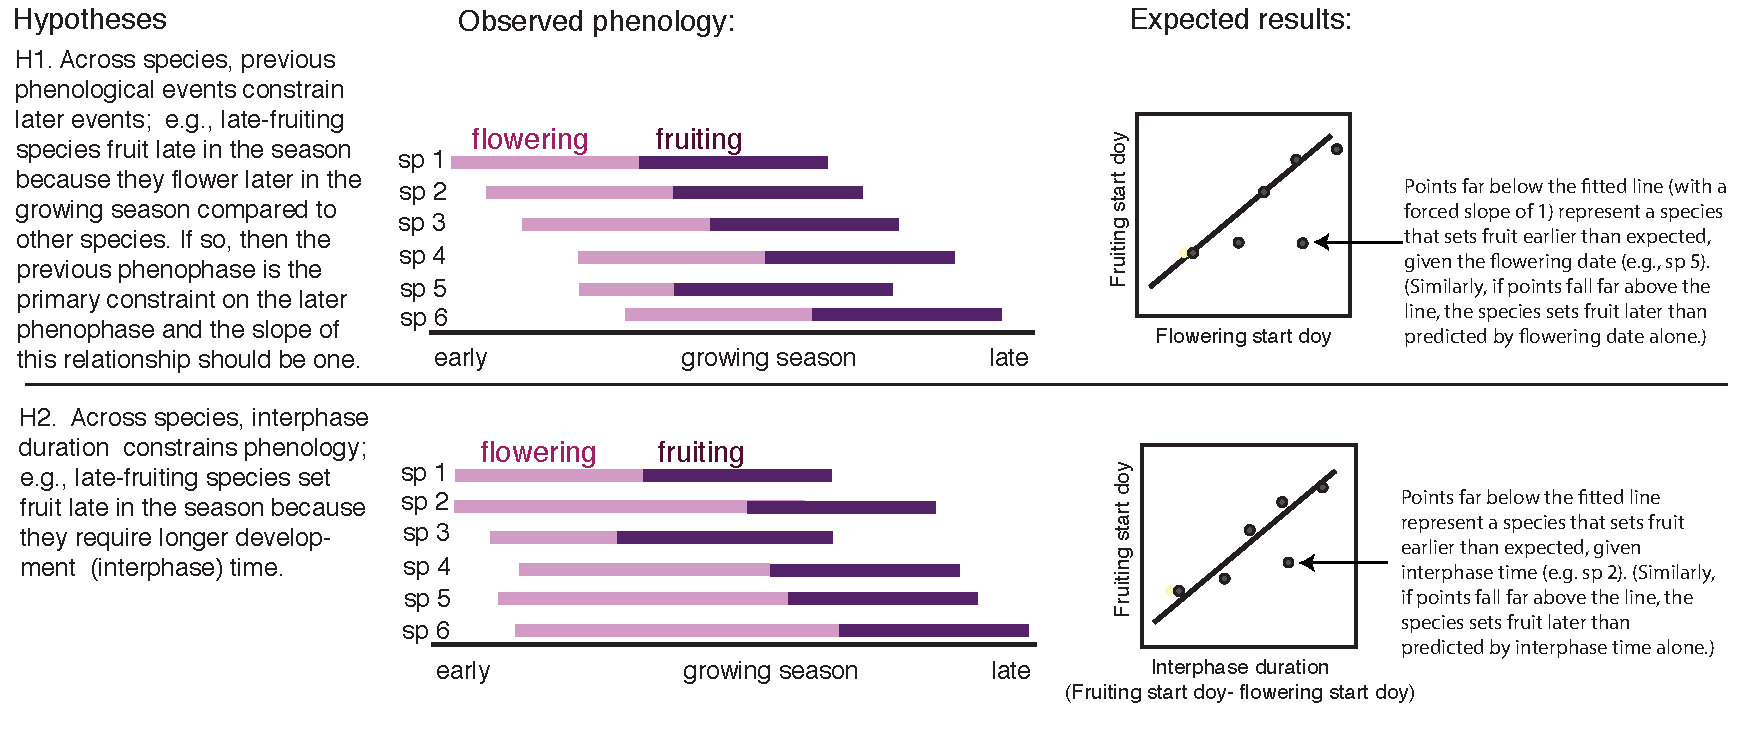
\includegraphics{../analyses/figures/hypotheses3.pdf} 
  \caption{\textbf{Hypotheses.} We show flowering and fruiting as examples of consecutive phenological events. We expected the same patterns for other consecutive events,such as leaf budburst and leafout. Inter-phenophase duration is the time between phenological events, e.g., the number of days between the start of flowering and the start of fruiting.} 
 \label{fig:hyp}
\end{figure}
 
\begin{figure}[h]
  \centering
  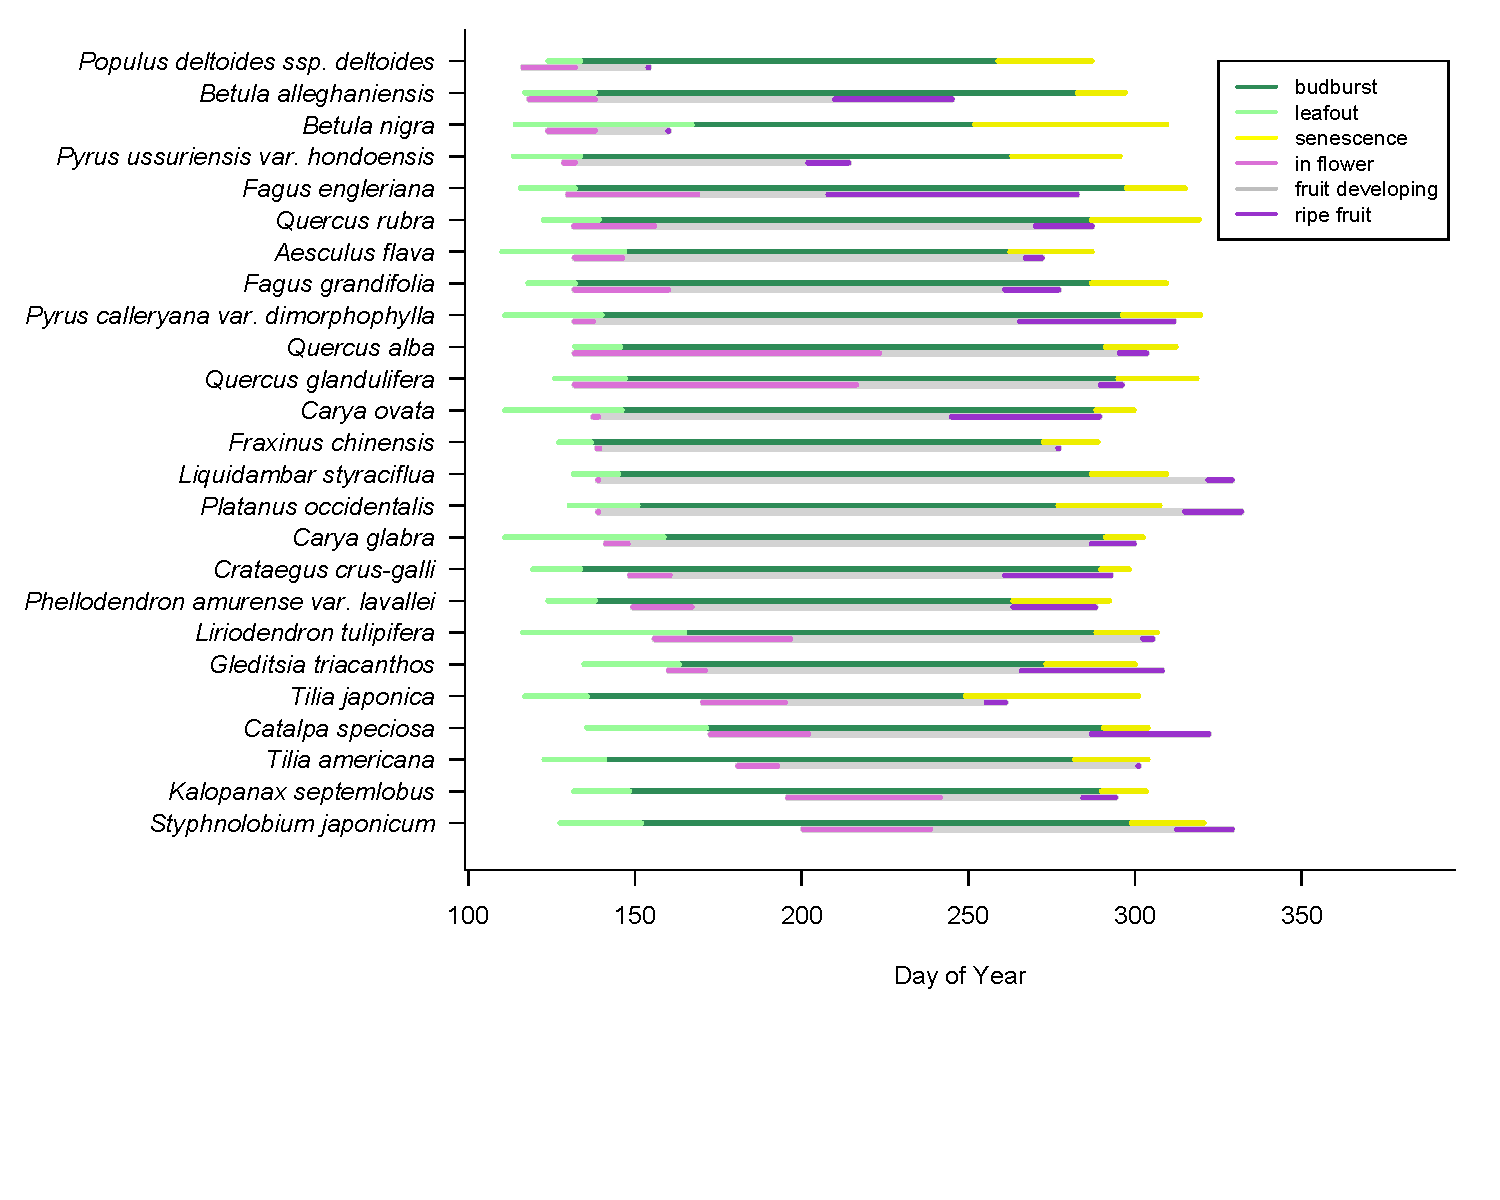
\includegraphics{../analyses/figures/grosea_repsort_ripefruit_legend.pdf}
  \caption{\textbf{Species' phenology during the 2015 growing season, ordered by mean first-flower dates.} Growth phenology is shown for budburst (from its mean start day-of-year to the mean start day-of-year for leafout, across all individuals within a species), leafout (from the mean day-of-year when fully-expanded leaves were first observed through the start of senescence), and senescence (from the mean day-of-year when leaves first began changing color through the mean day-of-year when more than 95 percent of leaves on the tree had changed color). Reproductive phenology is shown for flowering (from the mean day-of-year when flowers first appeared to the mean day-of-year when fruits first appeared, across all individuals within a species) and fruiting (from the mean day-of-year when fruits first appeared to the mean day-of-year when more than 95 percent of fruits were first observed as ripe).}
  \label{fig:focsp}
\end{figure}
  
  \begin{figure}[h]
  \centering
  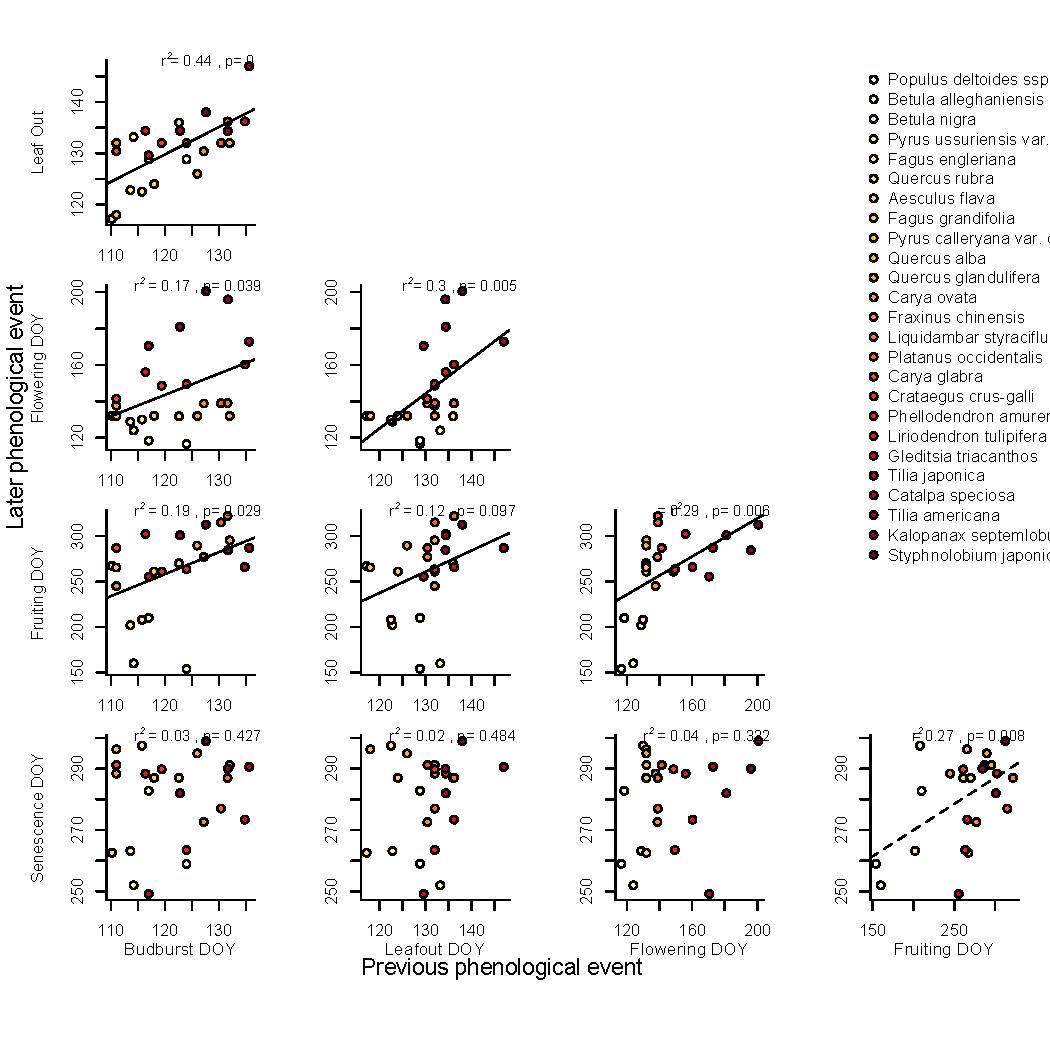
\includegraphics{../analyses/figures/latevearly_rp_col_legend_ROY_ripefruit.pdf}
  
  \caption{\textbf{Relationships among phenological stages across the 25 focal species.} Linear models were fit with the species-level mean day-of-year (DOY) of the later phenological stages as the response variable, and mean day-of-year of earlier stage as the explanatory variable. R\textsuperscript{2} and \textit{P}-value for each model are shown, with solid lines representing model fit when \textit{P}<0.05 and dashed lines representing model fit when 0.05<\textit{P}<0.10. Full model statistics are summarized in Table S1 in the Supplemental Materials. Species in the legend are ordered from early to late first-flower dates, as in Figure 2.} %EMW: Nice!
  \label{fig:latevearly}
\end{figure}
\begin{figure}[h]
  \centering
  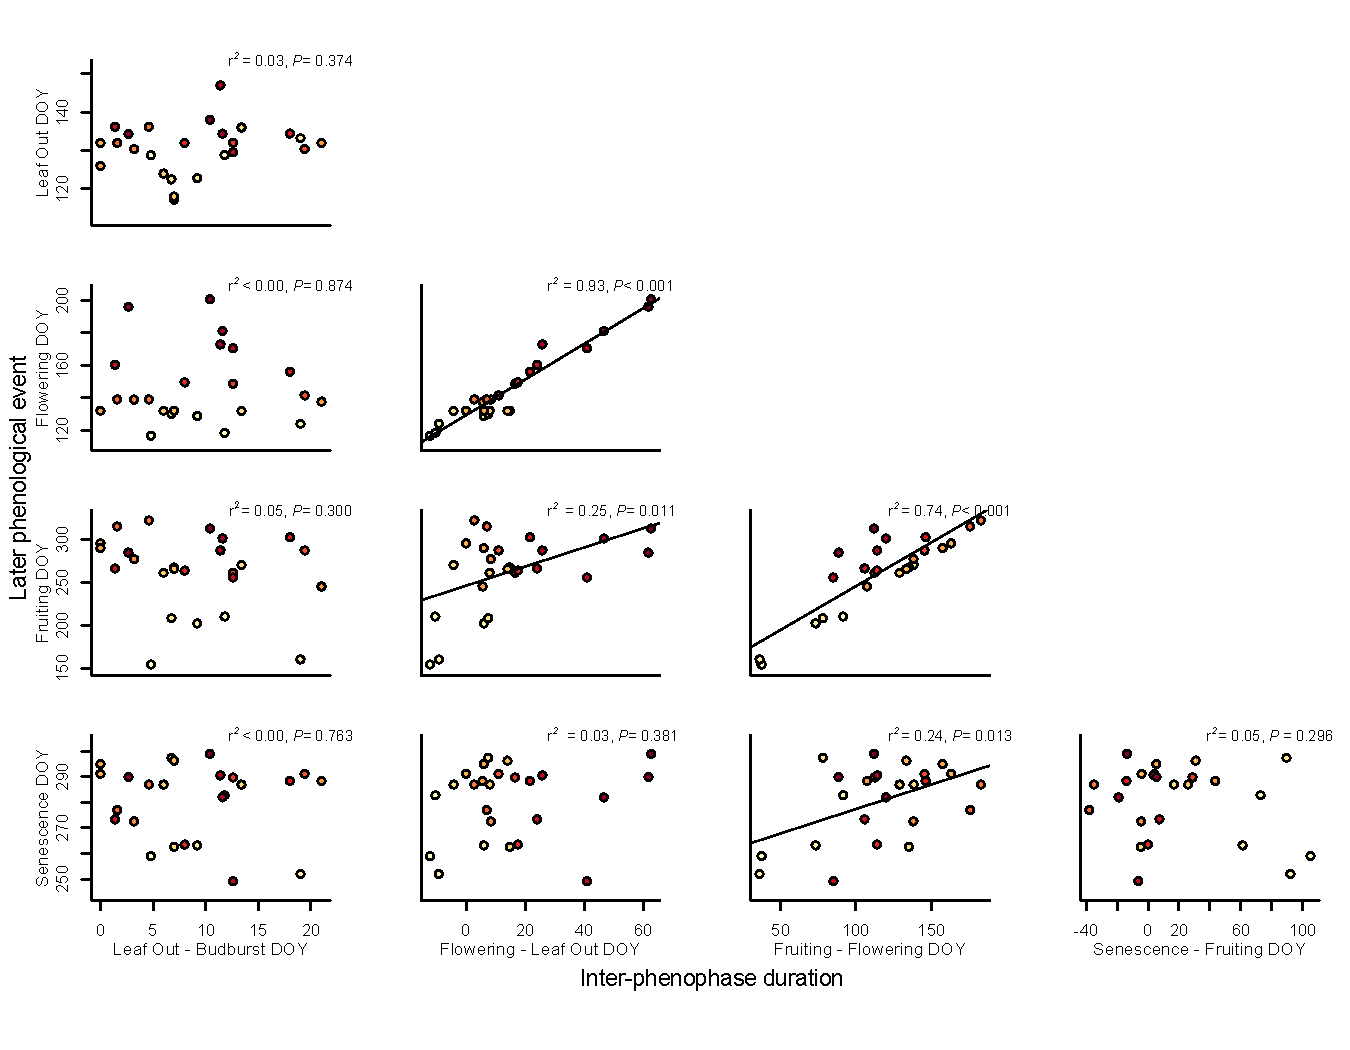
\includegraphics{../analyses/figures/adj_stagesmegaplot_col_YOR_ripefruit_lowertri.pdf}
  \caption{\textbf{Relationships among phenological stages and inter-phenophase duration across the 25 focal species.} Inter-phenophase duration is the time between the start of the earlier phenological event and the start of the later phenological event, e.g., the number of days between the species' mean start of flowering and its mean start of fruiting. Linear models were fit with the species-level mean day-of-year (DOY) of the later phenological stages as the response variable, and inter-phenophase duration as the explanatory variable. R\textsuperscript{2} and \textit{P}-value for each model are shown, with solid lines representing model fit when \textit{P}<0.05 and dashed lines representing model fit when 0.05<\textit{P}<0.10. Full model statistics are summarized in Table S1 in the Supplemental Materials. Species are color-coded as in Figure 3.}
  \label{fig:inter}
   \end{figure}


%%%%%%%%%%%%%%%%%%%%%%%%%%%%%%%%%%%%%%%%
\end{document}
%%%%%%%%%%%%%%%%%%%%%%%%%%%%%%%%%%%%%%%%
